%%%%%%%%%%%%%%%%%%%%%%%%%%%%%%%%%%%%%%%%%%%%%%%%%%%%%%%%%
%                         导言区                        %
%%%%%%%%%%%%%%%%%%%%%%%%%%%%%%%%%%%%%%%%%%%%%%%%%%%%%%%%%

\documentclass[13pt]{ctexart} % 文档类
\usepackage{geometry} % 设置页面
\usepackage{graphicx} % 插图片
\graphicspath{{C:/Users/zheng/Desktop/mcm-2021/mcmdocs/figs/}}
\renewcommand{\figurename}{Figure} % 设置标题 重命名为英文
\renewcommand{\tablename}{Table}
\renewcommand{\contentsname}{Contents}
\usepackage{changepage} % 设置摘要页缩减
\usepackage{fontspec} % 便于修改字体
\usepackage{fancyhdr} % 设置页眉页脚
\usepackage{lastpage}
\pagestyle{fancy} % 清空页眉页脚
\usepackage[shortlabels]{enumitem} % 设置列表缩进
\usepackage{titlesec} % 设置修改默认的section标题大小
\titleformat*{\section}{\LARGE}
\titleformat*{\subsection}{\Large}
\titleformat*{\subsubsection}{\Large}
\usepackage{amsmath} % 使用数学宏包
\usepackage{array} % 设置表格的列格式
\usepackage{booktabs} % 三线表宏包
\usepackage{etoolbox} % 设置参考文献不输出默认名
\patchcmd{\thebibliography}{\section*{\refname}}{}{}{} % 引入网站作为参考文献
\usepackage{url} % 设置等宽的代码字体
%\setmonofont{IBM Plex Mono}
% 建议这个,但我系统没这个字体,且懒得折腾了 windows用户请
\setmonofont{Courier New}
% 颜色
\usepackage{xcolor} % 代码高亮方案宏包
\usepackage{listings}
\definecolor{CPPLight}  {HTML} {686868}
\definecolor{CPPSteel}  {HTML} {888888}
\definecolor{CPPDark}   {HTML} {262626}
\definecolor{CPPBlue}   {HTML} {4172A3}
\definecolor{CPPGreen}  {HTML} {487818}
\definecolor{CPPBrown}  {HTML} {A07040}
\definecolor{CPPRed}    {HTML} {AD4D3A}
\definecolor{CPPViolet} {HTML} {7040A0}
\definecolor{CPPGray}   {HTML} {B8B8B8}
\lstset{
	basicstyle=\ttfamily,
	breaklines=true,
	framextopmargin=50pt,
	frame=bottomline,
	columns=fixed,
    %numbers=left,                                       % 在左侧显示行号
	frame=none,                                          % 不显示背景边框
	backgroundcolor=\color[RGB]{255,255,255},            % 设定背景颜色
	keywordstyle=\color[RGB]{40,40,255},                 % 设定关键字颜色
	numberstyle=\footnotesize\color{darkgray},           % 设定行号格式
	commentstyle=\itshape\color[RGB]{0,96,96},                % 设置代码注释的格式
	stringstyle=\slshape\color[RGB]{128,0,0},   % 设置字符串格式
	showstringspaces=false,                              % 不显示字符串中的空格
	language=python,                                     % 设置语言
	morekeywords={alignas,continute,friend,register,true,alignof,decltype,goto,
		reinterpret_cast,try,asm,defult,if,return,typedef,auto,delete,inline,short,
		typeid,bool,do,int,signed,typename,break,double,long,sizeof,union,case,
		dynamic_cast,mutable,static,unsigned,catch,else,namespace,static_assert,using,
		char,enum,new,static_cast,virtual,char16_t,char32_t,explict,noexcept,struct,
		void,export,nullptr,switch,volatile,class,extern,operator,template,wchar_t,
		const,false,private,this,while,constexpr,float,protected,thread_local,
		const_cast,for,public,throw,std},
	emph={map,set,multimap,multiset,unordered_map,unordered_set,numpy,graph,path,append,extend,
		unordered_multiset,unordered_multimap,vector,string,list,deque,
		array,stack,forwared_list,iostream,memory,shared_ptr,unique_ptr,
		random,bitset,ostream,istream,cout,cin,endl,move,default_random_engine,
		uniform_int_distribution,iterator,algorithm,functional,bing,numeric,},
	emphstyle=\color{CPPViolet},
}

%%%%%%%%%%%%%%%%%%%%%%%%%%%%%%%%%%%%%%%%%%%%%%%%%%%%%%%%%
%                         正文区                         %
%%%%%%%%%%%%%%%%%%%%%%%%%%%%%%%%%%%%%%%%%%%%%%%%%%%%%%%%%
\begin{document}
%%%%%%%%%%%%%%%%%%%%%%%%%%扉页%%%%%%%%%%%%%%%%%%%%%%%%%%
\newgeometry{top = 1cm, right = 2.54cm, left = 2.54cm, bottom = 2.54cm}
% 第一页的字体为times new roman
\setmainfont{Times New Roman}
\thispagestyle{empty}
% 扉页抬头
\begin{table}[h]
    \quad { }  \begin{minipage}[t]{5.5cm}
        % arraystretch 是调节列高
        \begin{tabular}[t]{>{\centering\arraybackslash}b{10em}}
            \fontsize{12pt}{10pt}\selectfont \textbf{Problem Chosen} \\ [2pt]
            {\color{red} \fontsize{20pt}{10pt}\selectfont ABC} % 问题
        \end{tabular}
    \end{minipage}
    \begin{minipage}[t]{5.2cm}
        \begin{tabular}[t]{>{\centering\arraybackslash}p{10em}}
            \fontsize{12pt}{10pt}\selectfont \textbf{2021}    \\ [-2pt]
            \fontsize{12pt}{10pt}\selectfont \textbf{MCM/ICM} \\ [-2pt]
            \fontsize{12pt}{10pt}\selectfont \textbf{Summary Sheet}
        \end{tabular}
    \end{minipage}
    \begin{minipage}[t]{3cm}
        \begin{tabular}[t]{>{\centering\arraybackslash}b{12em}}
            \fontsize{12pt}{10pt}\selectfont \textbf{Team Control Number} \\ [2pt]
            {\color{red} \fontsize{21pt}{10pt}\selectfont 2120710} % 队伍控制号
        \end{tabular}
    \end{minipage}
\end{table}
\vspace{-20pt}
\noindent{\rule{\textwidth}{0.5mm}}
% 大标题
{\centering\fontsize{18}{16}\selectfont\textbf{{标题}}

    % summary
    \vspace{10pt}
    \fontsize{13}{10}\selectfont\textbf{{Summary}}\par}
\vspace{10pt}

% summray正文
\fontsize{13}{12.5}\selectfont %summary正文字体 13 pt
\begin{adjustwidth}{1cm}{1cm}
    \indent { }{ }{ }{ }{ }{ }
    在这里写summary

    % 关键词
    \vspace{15pt}
    \textbf{key words} : 关键词1; 关键词2; 关键词3
\end{adjustwidth}

%%%%%%%%%%%%%%%%%%%%%%%%%%MEMO页%%%%%%%%%%%%%%%%%%%%%%%%%%
\newpage
% 开始写 memo 信
% 更换字体为 palatino 也可以不换
\setmainfont{texgyrepagella-regular.otf}
\newgeometry{left = 3.5cm, right = 3.5cm}
\thispagestyle{empty}
% memo标题+信息
{\centering \fontsize{18pt}{14pt}\selectfont \textbf{MEMO}\par}

\noindent FROM: Team {} 2120710 , MCM\\
\noindent To: The group of Governors\\
\noindent Date: January 28, 2019
% memo正文
\vspace{10pt}
\\
这里是memo正文。

% 信多出一页,清理页眉页脚
\thispagestyle{empty}
% 信的结尾
{\raggedleft
    Sincerely yours,\\
    MCM Team 2120710\par
}

%%%%%%%%%%%%%%%%%%%%%%%%%%目录页%%%%%%%%%%%%%%%%%%%%%%%%%%
\newpage
\thispagestyle{empty}
\tableofcontents
%%%%%%%%%%%%%%%%%%%%%%%%%%正文页%%%%%%%%%%%%%%%%%%%%%%%%%%
\newpage
% 目录页后面是第一页
\setcounter{page}{1}

% 开始写正文
% 设置正文的页边距
\newgeometry{top=3cm, left=3.5cm, right=3.5cm}
% 设置正文的页眉页脚
\fancyhf{}
\fancyhead[C]{ }
% 此处修改右上角页码
\fancyhead[R]{Page \thepage\ of \pageref{LastPage}}
\fancyhead[L]{Team \# 2120710}
\fancyfoot[C]{\bfseries\thepage}
%%%%%%%%%%%%%%%%%%%%%%%%%%%%%%%%%%%%%%%
%% Introduction
\textbf{\section{Introduction}}
% .1
\textbf{\subsection{Restatement of the Problem}}
Many people...Therefore we are facing the following problems:
\begin{itemize}
    \item aaaaaa
    \item bbbbbbb
\end{itemize}
% .2
\textbf{\subsection{Our Works}}
\begin{itemize}
    \item aaaaaa
    \item bbbbbbb
\end{itemize}
\fancyfoot[C]{\bfseries\thepage}
%%%%%%%%%%%%%%%%%%%%%%%%%%%%%%%%%%%%%%%
%% Assumptions and Notations
\textbf{\section{Assumptions and Notations}}
\vspace*{-10pt}
\textbf{\subsection{Assumptions}}
Due to the lack of necessary data, we make the following assumptions to help us perform modeling.
\begin{itemize}[itemsep=0.3ex, leftmargin=1.2cm]
    \item[1.] Inflow of drugs from outside of the five states are neglected.
    \item[2.] The microscopic behaviors of opioid transmission are ignored.
\end{itemize}
\textbf{\subsection{Notations}}
Here are all the notations and their meanings in this paper.
\begin{table}[h]
    \centering
    \vspace{3pt}
    \begin{tabular}{>{\centering\arraybackslash}p{5em}>{\centering\arraybackslash}p{30em}}
        \toprule % 绘制第一条线
        Symbol & Meaning                     \\ \midrule
        $t$    & Time                        \\
        $N$    & Total reported opioid cases \\
        \bottomrule
    \end{tabular}
\end{table}
%%%%%%%%%%%%%%%%%%%%%%%%%%%%%%%%%%%%%%%
%% Model Construction
\textbf{\section{Model Construction}}
blablablabla
%%%%%%%%%%%%%%%%%%%%%%%%%%%%%%%%%%%%%%%
%% Conclusion
\textbf{\section{Conclusion}}
We build a.....interesting findings:\cite{entroy}

\begin{itemize}
    \item aaaaaaa
    \item aaaaaaa
\end{itemize}

%%%%%%%%%%%%%%%%%%%%%%%%%%参考文献%%%%%%%%%%%%%%%%%%%%%%%%%%
% 因为不输出此部分到目录 \addcontentsline{}{}{}是添加此标题到目录
\newpage
\textbf{\section*{References}\addcontentsline{toc}{section}{References}}
\fancyhf{}
\fancyhead[R]{ }
\fancyhead[L]{ }
\bibliography{books}
\Large
\bibliographystyle{IEEEtran}
%%%%%%%%%%%%%%%%%%%%%%%%%%附录%%%%%%%%%%%%%%%%%%%%%%%%%%
\newpage
\textbf{\section*{Appendices}\addcontentsline{toc}{section}{Appendices for Code and Data}}
\fontsize{13pt}{12.5pt}\selectfont
Here is Code we used in our model, which python is the main development language.
\vspace{7pt}
\textbf{\subsection*{Appendices A}}
\begin {figure}[h]
\centering % 居中显示
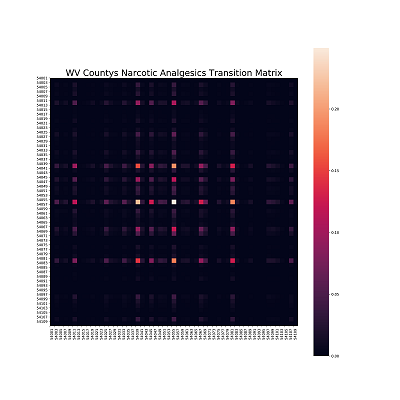
\includegraphics[width=15cm,height=12cm]{8.png}
\caption{Transition matrix for synthetic opioid spread rate in West Virginia} % 标题
\end {figure}

\end{document}